\documentclass[a4paper,12pt]{article}

%% Language and font encodings
\usepackage[english]{babel}
\usepackage[utf8]{inputenc}
\usepackage[T1]{fontenc}

%% Page size and margins
\usepackage[a4paper,top=2.5cm,bottom=2.5cm,left=3cm,right=3cm,marginparwidth=1.75cm]{geometry}

%% Core packages
\usepackage{amsmath}
\usepackage{amssymb}
\usepackage{graphicx}
\usepackage{tabularx}
\usepackage{booktabs}
\usepackage{float}
\usepackage{subcaption}
\usepackage[protrusion=true,expansion=false]{microtype}
\usepackage{xcolor}
\usepackage{enumitem}
\usepackage{array}
\usepackage{multirow}
\usepackage{longtable}
\definecolor{tcdBlue}{RGB}{5, 105, 185}
\definecolor{lightgray}{RGB}{245,245,245}

%% TikZ for architecture and flow diagrams
\usepackage{tikz}
\usetikzlibrary{positioning,shapes.geometric,arrows.meta,fit,calc,backgrounds}

%% Algorithm pseudocode
\usepackage{algorithm}
\usepackage{algpseudocode}
\algnewcommand\algorithmicinput{\textbf{Input:}}
\algnewcommand\Input{\item[\algorithmicinput]}

%% Code listings
\usepackage{listings}
\lstset{basicstyle=\small\ttfamily, backgroundcolor=\color{lightgray},
        frame=single, breaklines=true}

%% Hyperlinks
\usepackage[colorlinks=true,linkcolor=tcdBlue,citecolor=tcdBlue,urlcolor=tcdBlue]{hyperref}

%% Section heading style
\usepackage{titlesec}
\titleformat{\section}[hang]{\normalfont\Large\bfseries\color{tcdBlue}}{\thesection}{1em}{}
\titleformat{\subsection}[hang]{\normalfont\large\bfseries\color{tcdBlue}}{\thesubsection}{1em}{}
\titleformat{\subsubsection}[hang]{\normalfont\normalsize\bfseries}{\thesubsubsection}{1em}{}

\hyphenation{op-tical net-works semi-conduc-tor}

% ============================================================
\begin{document}
% ============================================================

\begin{titlepage}
\centering
\vspace*{2cm}

{\Huge\bfseries\color{tcdBlue}
Empirical Comparison of Reinforcement\\[0.3em]
Learning Algorithms Across Environments\\[0.3em]
of Increasing Complexity
\par}

\vspace{1.5cm}

{\large\bfseries
A Report Submitted in Partial Fulfilment of the Requirements\\
for the Degree of Master of Science in Computer Science
\par}

\vspace{2cm}

{\large
\textbf{Vinol Tauro}\\[0.3em]
Student Number: 25340566\\[0.3em]
School of Computer Science and Statistics\\
Trinity College Dublin
\par}

\vspace{2cm}

{\large June 2026\par}

\end{titlepage}

% ============================================================
\begin{abstract}
\noindent
This report presents a rigorous empirical comparison of four reinforcement learning algorithms across three environments of strictly increasing complexity: a custom $6\times6$ GridWorld, CartPole-v1, and MountainCar-v0 from OpenAI Gymnasium. The algorithms evaluated are tabular Q-Learning, Deep Q-Network (DQN) with the Double DQN correction, Advantage Actor-Critic (A2C), and Proximal Policy Optimisation (PPO). The study makes three contributions. First, it provides a clean comparative benchmark demonstrating that all four algorithms solve GridWorld and CartPole, with solution episodes ranging from 195 (PPO) to 9,798 (Q-Learning), a 50-fold difference reflecting the compounding advantages of continuous function approximation, off-policy replay, and multi-epoch updates. Second, it documents 44 implementation issues identified and corrected across the four algorithms, ranging from a tensor broadcasting error that silently zeroed all A2C policy gradients for 5,000 episodes, to a Q-value overestimation cascade, to a learning-rate schedule coupling that caused divergent training trajectories through the butterfly effect. Third, it empirically reproduces seven deep RL pathologies documented in the literature. These are Q-value overestimation \cite{van2016deep}, truncation bias \cite{pardo2018time}, reward hacking \cite{ng1999policy,forbes2025adops}, Monte Carlo return variance \cite{schulman2015high}, entropy coefficient sensitivity, replay buffer capacity effects \cite{zhang2019deeper,fedus2020revisiting}, and implementation sensitivity \cite{henderson2018deep,engstrom2020implementation}, each demonstrated using controlled ablation studies. MountainCar-v0 is not solved by any algorithm within the evaluated budgets. A2C is shown to fail at two structural levels: the zero-advantage fixed point (single environment) and the hard-exploration problem (vectorised $n_\text{envs}=16$, 1.024M steps, zero goals). The best results are PPO at mean $-151.8$ (4,816 goal discoveries, no regression) and Double DQN at a stable mean $-146.7$.
\end{abstract}

\tableofcontents
\newpage

% ============================================================
\section{Introduction}
% ============================================================

Reinforcement learning (RL) has produced remarkable results in recent years, from superhuman Go play \cite{silver2021reward} to the fine-tuning of large language models via RLHF, yet the field is frequently criticised for poor reproducibility and extreme sensitivity to implementation details \cite{henderson2018deep,engstrom2020implementation}. The gap between a correct algorithm as described in a paper and a correct implementation that actually learns is substantial, and that gap is rarely documented systematically.

This report addresses that gap directly. Rather than proposing a new algorithm, it takes four established algorithms: tabular Q-Learning \cite{watkins1992q}, DQN \cite{mnih2015human} with the Double DQN correction \cite{van2016deep}, A2C \cite{mnih2016asynchronous}, and PPO \cite{schulman2017proximal}. Each is implemented, debugged, and compared across three environments chosen to expose different algorithmic strengths and failure modes.

The three environments form a deliberate progression. \textbf{GridWorld} is a discrete, low-dimensional, dense-reward navigation task that any correct RL implementation should solve quickly. \textbf{CartPole-v1} introduces continuous state, stochastic dynamics, and a solved threshold requiring sustained performance over 100 episodes. This is a test of policy stability rather than just peak performance. \textbf{MountainCar-v0} introduces the hard-exploration problem: the reward is sparse and deceptive, the optimal policy requires counter-intuitive behaviour (drive backwards to build momentum), and random exploration almost never reaches the goal \cite{dann2022exploration}. Solving all three requires navigating a distinct set of challenges for each environment-algorithm pair.

The key contributions are:

\begin{enumerate}
  \item \textbf{A clean comparative benchmark} across 12 environment-algorithm combinations, with solved episode counts and performance statistics directly comparable across algorithms because all implementations share identical environments, reward functions, and evaluation protocols.

  \item \textbf{A documented audit of 44 implementation issues}, each classified by severity, root cause, and the specific experiment that revealed it. This audit constitutes a practical guide to the failure modes of these four algorithms.

  \item \textbf{Empirical reproduction of seven literature pathologies} using controlled ablations. Each pathology is demonstrated with a failing run, explained theoretically, corrected with a specific code change, and confirmed with a passing run.
\end{enumerate}

The remainder of this report is structured as follows. Section~\ref{sec:background} reviews the theoretical foundations and key literature. Section~\ref{sec:methodology} describes the experimental design and algorithm implementations. Section~\ref{sec:results} presents all results. Section~\ref{sec:debugging} documents the most significant implementation issues. Section~\ref{sec:discussion} interprets the findings. Section~\ref{sec:conclusion} concludes.

% ============================================================
\section{Background and Literature Review}
\label{sec:background}
% ============================================================

\subsection{Foundational Theory}

The Bellman optimality equation \cite{bellman1957dynamic} provides the mathematical foundation for all value-based RL. It establishes that the value of a state under an optimal policy decomposes recursively:
\begin{equation}
  V^*(s) = \max_a \left[ r(s,a) + \gamma \sum_{s'} P(s'|s,a)\, V^*(s') \right]
\end{equation}
Without this decomposition, iterative value updates could not be guaranteed to converge to global optima.

Q-Learning \cite{watkins1992q} extends this to model-free settings by learning action-value estimates $Q(s,a) \approx Q^*(s,a)$ directly from experience. Watkins and Dayan proved convergence under two conditions: all state-action pairs must be visited infinitely often, and learning rates must satisfy $\sum_t \alpha_t = \infty$ and $\sum_t \alpha_t^2 < \infty$. This convergence guarantee holds for the tabular setting; function approximation removes it but dramatically extends scalability.

Temporal difference learning \cite{sutton1988learning} bridges Monte Carlo methods and dynamic programming. The $\lambda$ parameter interpolates between single-step TD (TD(0), low variance, high bias) and full Monte Carlo ($\lambda=1$, zero bias, high variance), forming the theoretical basis of GAE \cite{schulman2015high}.

The Policy Gradient Theorem \cite{sutton2018reinforcement} proves that the gradient of expected return with respect to policy parameters can be computed without differentiating the state distribution. This result makes A2C and PPO mathematically tractable for continuous and discrete control alike.

\subsection{Deep Q-Networks}

DQN \cite{mnih2015human} demonstrated that deep neural networks could stably learn control policies by introducing two stabilising mechanisms. \textbf{Experience replay} stores transitions $(s, a, r, s')$ in a circular buffer and samples uniformly, breaking temporal correlations and satisfying the i.i.d.\ assumption required for stochastic gradient descent. \textbf{Target networks} freeze a copy of the online network for multiple update steps, preventing the moving-target problem. Without these mechanisms, non-linear function approximation in off-policy RL falls into the \textit{deadly triad} of instability: the combination of function approximation, bootstrapping, and off-policy learning \cite{sutton2018reinforcement}.

Despite this success, standard DQN suffers from systematic Q-value overestimation. The TD target $y = r + \gamma \max_{a'} Q(s', a';\, \theta^-)$ uses the same network to both select and evaluate the best next action. Because $\mathbb{E}[\max_a \hat{Q}(s,a)] \geq \max_a \mathbb{E}[\hat{Q}(s,a)]$ by Jensen's inequality, the maximum over noisy estimates is biased upward. Double DQN \cite{van2016deep} decouples selection from evaluation:
\begin{equation}
  y = r + \gamma\, Q\!\left(s',\, \arg\max_{a'} Q(s', a';\, \theta);\, \theta^-\right)
\end{equation}
This study reproduces the overestimation plateau empirically (Section~\ref{sec:dqn_bugs}) and confirms the correction.

Replay buffer size is a critical hyperparameter \cite{zhang2019deeper}. A buffer too small fills with recent, correlated transitions, overwriting the rare high-reward trajectories needed for recovery. A buffer too large introduces stale data, slowing propagation of newly discovered transitions. Fedus et al.\ \cite{fedus2020revisiting} further show that the optimal buffer size depends on the ratio of learning rate to environment stationarity.

\subsection{Actor-Critic Methods}

A2C \cite{mnih2016asynchronous} combines a policy network (actor) with a value network (critic) under the advantage function $A(s,a) = Q(s,a) - V(s)$. The critic provides a state-dependent baseline that reduces policy gradient variance, while the actor moves in the direction that increases the probability of positive-advantage actions.

Generalised Advantage Estimation (GAE) \cite{schulman2015high} addresses the bias-variance tradeoff in advantage estimation. GAE computes the exponentially-weighted $\lambda$-return:
\begin{equation}
  \hat{A}_t^{\text{GAE}(\gamma,\lambda)} = \sum_{k=0}^{\infty} (\gamma\lambda)^k \delta_{t+k}, \quad \delta_t = r_t + \gamma V(s_{t+1}) - V(s_t)
\end{equation}
with $\lambda=0.95$ as the standard setting. This study demonstrates that replacing GAE with Monte Carlo returns in A2C causes the critic to converge to the bad policy's value function, eliminating useful advantage signals (Section~\ref{sec:ac_bugs}).

\subsection{Proximal Policy Optimisation}

PPO \cite{schulman2017proximal} addresses the instability of large policy updates by optimising a clipped surrogate objective:
\begin{equation}
  \mathcal{L}^{\text{CLIP}}(\theta) = \mathbb{E}_t\!\left[\min\!\left(r_t(\theta)\hat{A}_t,\ \text{clip}(r_t(\theta), 1-\varepsilon, 1+\varepsilon)\hat{A}_t\right)\right]
\end{equation}
where $r_t(\theta) = \pi_\theta(a_t|s_t)/\pi_{\theta_\text{old}}(a_t|s_t)$. The clip prevents updates that move the policy too far from the behaviour policy. The combined loss with entropy bonus and value function loss is:
\begin{equation}
  \mathcal{L}(\theta) = \mathcal{L}^{\text{CLIP}}(\theta) - c_1 \mathcal{L}^{\text{VF}}(\theta) + c_2 \mathcal{H}[\pi_\theta(s_t)]
\end{equation}

Engstrom et al.\ \cite{engstrom2020implementation} identify orthogonal weight initialisation, advantage normalisation, observation normalisation, and learning rate scheduling as critical implementation details. All are implemented in this study's PPO.

\subsection{Reward Shaping}

MountainCar-v0 \cite{moore1990efficient} presents a canonical sparse-reward challenge: the car receives $-1$ at every step regardless of position. Without additional signal, random exploration almost never reaches the goal within 200 steps \cite{dann2022exploration}.

Potential-based reward shaping \cite{ng1999policy} adds $F(s,s') = \gamma\Phi(s') - \Phi(s)$ to the environment reward, where $\Phi$ is a potential function. Ng et al.\ prove this transformation preserves the optimal policy. The shaping used in this study, specifically $r_{\text{shaped}} = h(s) + 100v^2 - 1$ where $h(s)$ is normalised height, is \emph{not} potential-based, as it adds a kinetic energy term that depends on velocity rather than solely on position differences. This violates the invariance theorem and can in principle alter the optimal policy. Forbes et al.\ \cite{forbes2025adops} confirm in contemporary work that non-potential-based shaping remains vulnerable to reward hacking, where the agent exploits the shaped signal without solving the original task.

Hindsight Experience Replay \cite{andrychowicz2017hindsight} offers a theoretically cleaner alternative: replaying failed trajectories with the achieved state as the artificial goal, avoiding reward modification entirely.

\subsection{Exploration and the Hard-Exploration Problem}

The exploration-exploitation tradeoff governs all RL agents, but its difficulty scales sharply with reward sparsity. In CartPole, the reward is dense ($+1$ per step the pole is upright), so any exploratory action provides feedback and $\varepsilon$-greedy exploration suffices. In MountainCar, the reward is $-1$ every step regardless of position, creating a completely flat exploration landscape.

Dann et al.\ \cite{dann2022exploration} provide strict mathematical bounds on the sample complexity of myopic exploration policies. For MDPs with sparse rewards, $\varepsilon$-greedy scales quadratically with the inverse of the exploration gap. For MountainCar specifically, the optimal trajectory requires a sustained sequence of left-push actions to build kinetic energy before a rightward push achieves the goal. With $\varepsilon = 0.001$ (the minimum exploration rate after decay), the probability of a random walk producing this coordinated sequence over 50 or more consecutive steps is of order $\varepsilon^{50} \approx 10^{-150}$, which is effectively zero.

This mathematical reality explains why reward shaping is not merely convenient but mandatory for MountainCar: without shaping, no algorithm in this study makes progress from random initialisation. With shaping ($h(s) + 100v^2 - 1$), the reward gradient points toward high-momentum states regardless of goal proximity, providing a navigable landscape for gradient-based optimisation.

However, shaping introduces its own failure mode. Because the shaped reward rewards velocity independently of position, the optimal policy under the shaped reward can involve oscillating at high velocity near the valley bottom without crossing the goal threshold. This is the non-potential-based shaping risk documented by Ng et al.\ \cite{ng1999policy} and empirically confirmed in this study for tabular Q-Learning (Section~\ref{sec:shaping_bugs}).

\subsection{Reproducibility in Deep RL}

Henderson et al.\ \cite{henderson2018deep} demonstrated that reported deep RL results are frequently non-reproducible: minor changes to network architecture, random seed, or batch size produce performance variations larger than the reported improvement over a baseline. Engstrom et al.\ \cite{engstrom2020implementation} localise this to PPO, showing that specific code-level details --- orthogonal initialisation, advantage normalisation, global reward scaling --- determine performance more than the clipped objective itself.

Lynnerup et al.\ \cite{lynnerup2020survey} confirm through a systematic survey across real-world robotic benchmarks that irreproducibility arises from intrinsic algorithmic variance, environment stochasticity, and opaque hyperparameter tuning. They advocate for rigorous statistical evaluation and standardised reporting, exactly the methodology adopted in this study's ablation protocol.

This study confirms Henderson et al.'s finding in a new context (Section~\ref{sec:ppo_bugs}): two runs of the same PPO configuration with \texttt{N\_EPISODES} differing by 4,000, which changes the learning rate at every step through the LR schedule formula, produced 4,816 goals versus approximately 95 goals, a 50-fold difference attributable entirely to trajectory divergence from the butterfly effect.

Pardo et al.\ \cite{pardo2018time} identify truncation bias as a systematic error in RL implementations. When an episode times out, the correct bootstrap target is $V(s_T)$, not zero. Treating timeout as a true terminal injects an artificial value cliff at step $T$ that corrupts the value function backward through time. This bias is fixed in both the A2C and PPO implementations in this study.

% ============================================================
\section{Methodology}
\label{sec:methodology}
% ============================================================

\subsection{Environments}

\subsubsection{GridWorld}

A custom $6\times6$ discrete grid with one goal state, one start state, and wall penalties. The agent receives $+10$ for reaching the goal, $-0.1$ per step, and $-1$ for hitting a wall. Episodes terminate at the goal or after 200 steps. The state space is 36 discrete states; the action space is 4 directions.

\subsubsection{CartPole-v1}

The OpenAI Gymnasium CartPole-v1 environment \cite{brockman2016openai}. State: $(x, \dot{x}, \theta, \dot{\theta})$. Actions: $\{0,1\}$. Reward: $+1$ per step the pole remains upright. Solved threshold: mean reward $\geq 195$ over 100 consecutive episodes. Episode terminates when the pole angle exceeds $\pm12°$, the cart position exceeds $\pm2.4$, or after 500 steps.

\subsubsection{MountainCar-v0}

The classic hard-exploration benchmark introduced by Moore \cite{moore1990efficient}. State: $(x, v)$ where $x \in [-1.2, 0.6]$ and $v \in [-0.07, 0.07]$. Actions: $\{0,1,2\}$ (push left, neutral, push right). Reward: $-1$ per step. Solved threshold: mean reward $\geq -110$ over 100 consecutive episodes. Episode truncates after 200 steps.

\textbf{Reward shaping.} All deep RL methods use:
\begin{equation}
  r_{\text{shaped}}(s_{t+1}) = \frac{(x+1.2)}{1.8} \cdot 2 + 100v^2 - 1 + \mathbf{1}[\text{goal}] \cdot r_{\text{bonus}}
\end{equation}
The goal bonus is $r_{\text{bonus}} = +10$ for PPO/A2C and $+2$ for DQN. Tabular Q-Learning uses raw rewards only (see Section~\ref{sec:shaping_bugs}).

\subsection{Network Architectures}

All deep RL algorithms use fully-connected networks with orthogonal weight initialisation \cite{saxe2013exact}. Figure~\ref{fig:arch} shows the two architectural variants.

\begin{figure}[H]
\centering
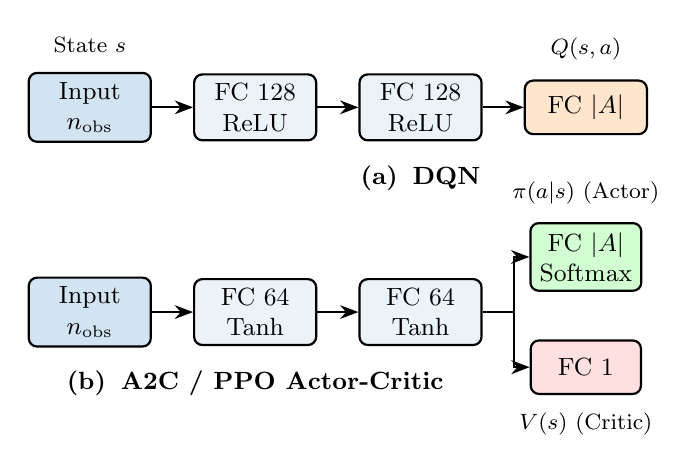
\begin{tikzpicture}[
  blk/.style={draw, rectangle, rounded corners=3pt, minimum width=1.55cm,
              minimum height=0.68cm, font=\small, fill=tcdBlue!8, align=center},
  head/.style={blk, minimum width=1.4cm},
  ann/.style={font=\footnotesize, align=center},
  >=Stealth, thick
]
%% ── DQN ─────────────────────────────────────────────────────
\node[blk, fill=tcdBlue!18] (d0) at (0,   0) {Input\\$n_\text{obs}$};
\node[blk]                  (d1) at (2.1, 0) {FC 128\\ReLU};
\node[blk]                  (d2) at (4.2, 0) {FC 128\\ReLU};
\node[blk, fill=orange!20]  (d3) at (6.3, 0) {FC $|A|$};
\draw[->] (d0)--(d1); \draw[->] (d1)--(d2); \draw[->] (d2)--(d3);
\node[ann, above=0.12cm of d0] {State $s$};
\node[ann, above=0.12cm of d3] {$Q(s,a)$};
\node[font=\small\bfseries, below=0.18cm of d2] {(a)\enspace DQN};

%% ── Actor-Critic ──────────────────────────────────────────────
\node[blk, fill=tcdBlue!18] (a0) at (0,   -2.6) {Input\\$n_\text{obs}$};
\node[blk]                  (a1) at (2.1, -2.6) {FC 64\\Tanh};
\node[blk]                  (a2) at (4.2, -2.6) {FC 64\\Tanh};
\node[head, fill=green!18]  (aa) at (6.3, -1.9) {FC $|A|$\\Softmax};
\node[head, fill=red!12]    (ac) at (6.3, -3.3) {FC 1};
\draw[->] (a0)--(a1); \draw[->] (a1)--(a2);
\draw[->] (a2.east) -- ++(0.4,0) |- (aa.west);
\draw[->] (a2.east) -- ++(0.4,0) |- (ac.west);
\node[ann, above=0.1cm of aa] {$\pi(a|s)$ (Actor)};
\node[ann, below=0.1cm of ac] {$V(s)$ (Critic)};
\node[font=\small\bfseries, below=0.18cm of a1] {(b)\enspace A2C / PPO Actor-Critic};
\end{tikzpicture}
\caption{Network architectures used in this study. (a)~DQN: two hidden layers of 128 units with ReLU activations mapping the state to per-action Q-values. For CartPole the output has 2 units; for MountainCar, 3. (b)~A2C/PPO: two shared hidden layers of 64 units with Tanh activations, branching into a softmax policy head (actor) and a scalar value head (critic). All weights use orthogonal initialisation with gain $\sqrt{2}$.}
\label{fig:arch}
\end{figure}

\subsection{Algorithm Implementations and Pseudocode}

All algorithms are implemented in Python~3 with PyTorch and Gymnasium. Random seed 42 is fixed throughout.

\subsubsection{Tabular Q-Learning}

Algorithm~\ref{alg:ql} gives the pseudocode. GridWorld uses raw environment states; MountainCar uses $40\times40$ uniform discretisation over position and velocity (1,600 states).

\begin{algorithm}[H]
\caption{Tabular Q-Learning}
\label{alg:ql}
\begin{algorithmic}[1]
\Input $\alpha$ (learning rate), $\gamma$ (discount), $\varepsilon_0, \varepsilon_{\min}, \varepsilon_{\text{decay}}$
\State Initialise $Q(s,a) \leftarrow 0$ for all $s, a$;\enspace $\varepsilon \leftarrow \varepsilon_0$
\For{episode $= 1, \ldots, N$}
  \State $s \leftarrow$ initial state
  \Repeat
    \State $a \leftarrow \begin{cases} \text{Uniform}(A) & \text{with prob } \varepsilon \\ \arg\max_{a'} Q(s,a') & \text{otherwise} \end{cases}$
    \State Execute $a$;\enspace observe $r, s', \text{done}$
    \State $Q(s,a) \;\mathrel{+}=\; \alpha\!\left[r + \gamma \max_{a'} Q(s',a')\cdot\mathbf{1}[\neg\text{done}] - Q(s,a)\right]$
    \State $s \leftarrow s'$
  \Until{done}
  \State $\varepsilon \leftarrow \max\!\left(\varepsilon_{\min},\; \varepsilon\cdot\varepsilon_{\text{decay}}\right)$
\EndFor
\end{algorithmic}
\end{algorithm}

\subsubsection{Deep Q-Network (DQN)}

Network architecture: $n_{\text{obs}} \to 128 \to 128 \to n_{\text{actions}}$ with ReLU activations, Huber loss, and AdamW optimiser with AMSGrad. Algorithm~\ref{alg:ddqn} highlights the Double DQN target computation that decouples action selection from evaluation.

\begin{algorithm}[H]
\caption{Double DQN --- Optimise Step}
\label{alg:ddqn}
\begin{algorithmic}[1]
\Input Online network $\theta$, target network $\theta^-$, replay buffer $\mathcal{D}$
\State Sample minibatch $\{(s_i, a_i, r_i, s'_i)\}_{i=1}^{B}$ from $\mathcal{D}$
\For{each transition $(s_i, a_i, r_i, s'_i)$}
  \State $a^* \leftarrow \arg\max_{a'} Q(s'_i, a';\; \theta)$ \Comment{selection by online net}
  \State $y_i \leftarrow r_i + \gamma\, Q(s'_i, a^*;\; \theta^-)$ \Comment{evaluation by target net}
\EndFor
\State $\mathcal{L} \leftarrow \tfrac{1}{B}\sum_i \text{Huber}\!\left(Q(s_i,a_i;\theta) - y_i\right)$
\State Update $\theta$ via gradient descent on $\mathcal{L}$
\If{$\text{steps} \bmod T_{\text{hard}} = 0$} $\theta^- \leftarrow \theta$ \EndIf
\end{algorithmic}
\end{algorithm}

\subsubsection{Advantage Actor-Critic (A2C)}

Separate actor and critic networks, each $n_{\text{obs}} \to 64 \to 64$ with Tanh activations. GAE($\lambda=0.95$) advantage estimation with truncation-aware bootstrap. Separate Adam optimisers: actor LR $= 3\times10^{-4}$, critic LR $= 1\times10^{-4}$. Gradient norm clipping to 0.5.

\subsubsection{Proximal Policy Optimisation (PPO)}

Architecture identical to A2C. Algorithm~\ref{alg:ppo} gives the update step. Learning rate decays from $3\times10^{-4}$ to a floor of $5\times10^{-5}$ over a fixed 8,000 decay steps, independent of total episode count. Update every 1,024 environment steps; 10 epochs per update; minibatch size 64. Policy clip $\varepsilon=0.2$. No value function clipping.

\begin{algorithm}[H]
\caption{PPO --- Policy Update}
\label{alg:ppo}
\begin{algorithmic}[1]
\Input Policy $\pi_{\theta_{\text{old}}}$, collected buffer of $T$ transitions
\State Compute advantages $\hat{A}_t$ via GAE($\gamma=0.99, \lambda=0.95$)
\State Normalise: $\hat{A}_t \leftarrow (\hat{A}_t - \mu_A)/(\sigma_A + \varepsilon)$
\For{epoch $= 1, \ldots, K$} \Comment{$K=10$ in this study}
  \For{each minibatch of size $M$}
    \State $r_t(\theta) \leftarrow \pi_\theta(a_t|s_t)\;/\;\pi_{\theta_{\text{old}}}(a_t|s_t)$
    \State $\mathcal{L}^{\text{CLIP}} \leftarrow -\mathbb{E}\!\left[\min\!\left(r_t\hat{A}_t,\;\text{clip}(r_t, 1-\varepsilon, 1+\varepsilon)\hat{A}_t\right)\right]$
    \State $\mathcal{L}^{\text{VF}} \leftarrow \tfrac{1}{2}\mathbb{E}\!\left[(V_\theta(s_t) - R_t)^2\right]$
    \State $\mathcal{L} \leftarrow \mathcal{L}^{\text{CLIP}} + c_1\mathcal{L}^{\text{VF}} - c_2\mathcal{H}[\pi_\theta]$ \Comment{$c_1=0.5,\; c_2=0.01$}
    \State Update $\theta$ via Adam; clip gradient norm to 0.5
  \EndFor
\EndFor
\State $\theta_{\text{old}} \leftarrow \theta$
\end{algorithmic}
\end{algorithm}

\subsection{Data Collection Strategies}

A key architectural distinction between the algorithms is how they collect and reuse experience (Figure~\ref{fig:rollout}). This difference directly determines sample efficiency on CartPole and structural failure modes on MountainCar.

\begin{figure}[H]
\centering
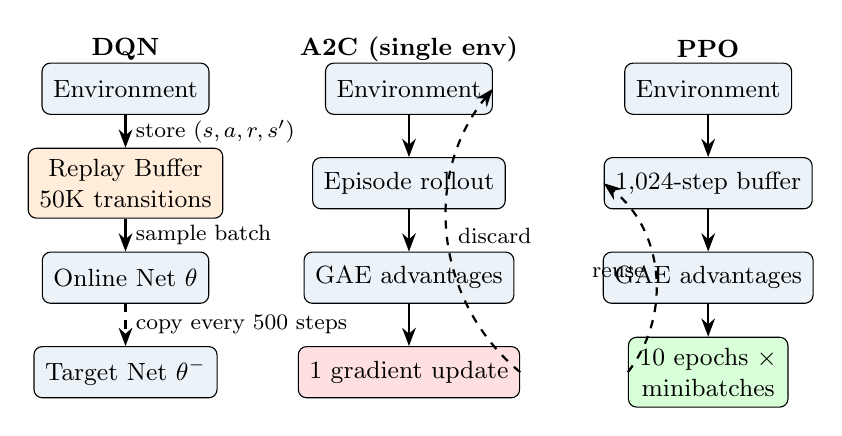
\begin{tikzpicture}[
  box/.style={draw, rounded corners=3pt, fill=tcdBlue!8, minimum height=0.65cm,
              font=\small, align=center, inner sep=4pt},
  buf/.style={box, fill=orange!15, minimum width=2.2cm},
  arr/.style={->, >=Stealth, thick},
  lab/.style={font=\small\bfseries}
]
%% DQN column
\node[lab]         at (1.4, 0.5)  {DQN};
\node[box]         (de) at (1.4, 0)   {Environment};
\node[buf]         (db) at (1.4,-1.2) {Replay Buffer\\50K transitions};
\node[box]         (dn) at (1.4,-2.4) {Online Net $\theta$};
\node[box]         (dt) at (1.4,-3.6) {Target Net $\theta^-$};
\draw[arr] (de.south) -- (db.north) node[midway,right,font=\footnotesize]{store $(s,a,r,s')$};
\draw[arr] (db.south) -- (dn.north) node[midway,right,font=\footnotesize]{sample batch};
\draw[arr,dashed] (dn.south) -- (dt.north) node[midway,right,font=\footnotesize]{copy every 500 steps};

%% A2C column
\node[lab]         at (5.0, 0.5)  {A2C (single env)};
\node[box]         (ae) at (5.0, 0)   {Environment};
\node[box]         (ar) at (5.0,-1.2) {Episode rollout};
\node[box]         (au) at (5.0,-2.4) {GAE advantages};
\node[box, fill=red!12] (ag) at (5.0,-3.6) {1 gradient update};
\draw[arr] (ae)--(ar); \draw[arr] (ar)--(au); \draw[arr] (au)--(ag);
\draw[arr, dashed, bend left=45] (ag.east) to node[right,font=\footnotesize]{discard} (ae.east);

%% PPO column
\node[lab]         at (8.8, 0.5)  {PPO};
\node[box]         (pe) at (8.8, 0)   {Environment};
\node[box]         (pb) at (8.8,-1.2) {1,024-step buffer};
\node[box]         (pa) at (8.8,-2.4) {GAE advantages};
\node[box, fill=green!15] (pg) at (8.8,-3.6) {10 epochs $\times$\\minibatches};
\draw[arr] (pe)--(pb); \draw[arr] (pb)--(pa); \draw[arr] (pa)--(pg);
\draw[arr, dashed, bend right=45] (pg.west) to node[left,font=\footnotesize]{reuse} (pb.west);
\end{tikzpicture}
\caption{Data collection and update strategies. DQN (left) stores all transitions in a large replay buffer and samples randomly, enabling indefinite data reuse but requiring a separate target network for stability. A2C (centre) collects one episode, computes advantages, applies one gradient update, then discards the data. PPO (right) collects 1,024 steps, then reuses the same batch across 10 epochs of minibatch updates before discarding. PPO's multi-epoch reuse is why rare goal transitions have disproportionate influence compared to A2C.}
\label{fig:rollout}
\end{figure}

\subsection{Evaluation Protocol}

All algorithms are evaluated on raw (unshaped) rewards throughout training. A run is classified as \textit{solved} when the mean reward over 100 consecutive episodes meets or exceeds the environment's threshold. At training completion, a final 20-episode test with the greedy/deterministic policy is recorded.

% ============================================================
\section{Results}
\label{sec:results}
% ============================================================

\subsection{GridWorld}

Q-Learning solves GridWorld in 3,000 episodes, achieving a 100\% goal rate in the final 100 episodes with mean steps of 10.0 and mean reward of $9.07 \pm 0.17$. The agent exhibits the classic exploration-exploitation tradeoff: initial random exploration ($\varepsilon=1.0$) discovers the goal via random walk, and the Q-table then concentrates value along the shortest path as $\varepsilon$ decays.

\begin{figure}[H]
\centering
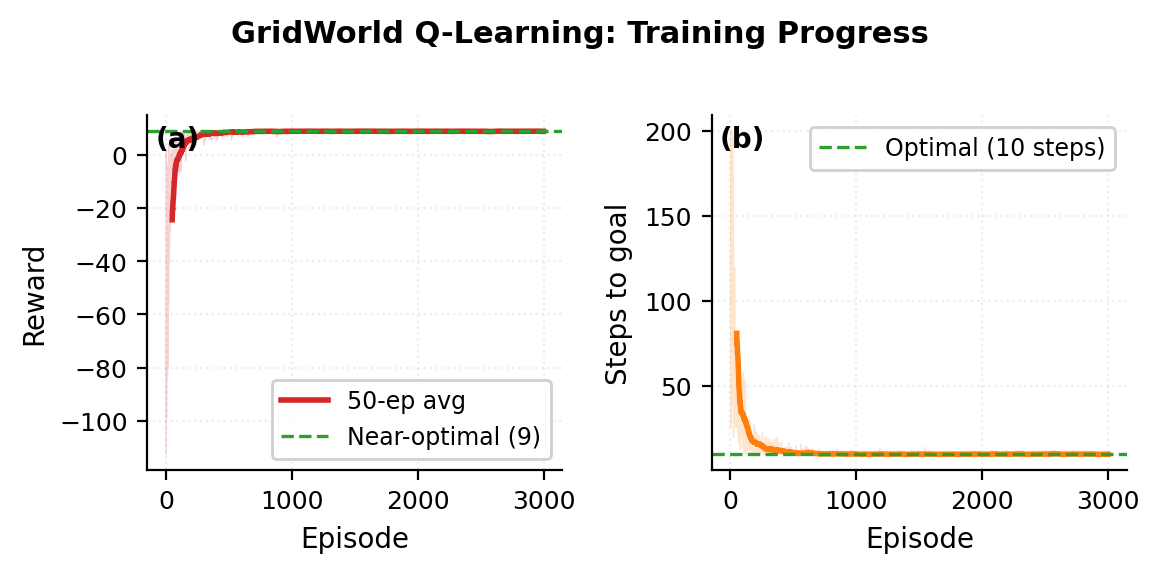
\includegraphics[width=\linewidth]{figures/fig_gridworld_training.png}
\caption{GridWorld Q-Learning training. (a)~Per-episode reward with 50-episode moving average, converging to the near-optimal score of 9. (b)~Steps to reach the goal, showing rapid convergence to the 10-step optimal path.}
\label{fig:gridworld}
\end{figure}

\begin{figure}[H]
\centering
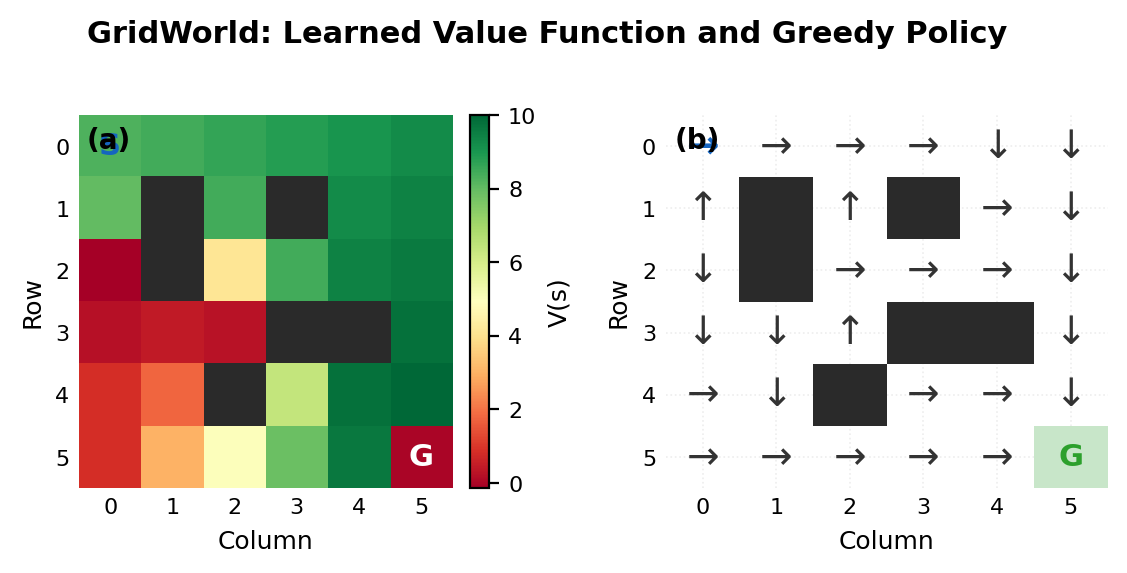
\includegraphics[width=\linewidth]{figures/fig_gridworld_policy.png}
\caption{GridWorld: learned value function and greedy policy after 3,000 training episodes. (a)~State value function $V(s) = \max_a Q(s,a)$; darkened cells are walls. High values appear along the shortest path to goal~G. (b)~Greedy policy $\pi(s) = \arg\max_a Q(s,a)$; arrows show the direction of maximum Q-value. Start state S is marked in blue.}
\label{fig:gridworld_policy}
\end{figure}

\subsection{CartPole}

All four algorithms solve CartPole. Table~\ref{tab:cartpole} summarises the results.

\begin{table}[H]
\centering
\caption{CartPole-v1 results. ``Solved at'' is the episode where the 100-episode rolling mean first exceeds 195. All runs use the same random seed.}
\label{tab:cartpole}
\begin{tabularx}{\linewidth}{lXXXX}
\toprule
\textbf{Algorithm} & \textbf{Solved at ep.} & \textbf{Mean (last 100)} & \textbf{Success rate} & \textbf{Key insight} \\
\midrule
Q-Learning & 9,798  & $195.0 \pm 36.8$  & 41/100 & Discretisation bottleneck \\
DQN        & 225    & $199.0 \pm 58.6$  & 49/100 & Sample-efficient off-policy \\
A2C        & 1,175  & $195.3 \pm 83.2$  & 43/100 & After advantage fix \\
PPO        & \textbf{195}    & $197.1 \pm 117.8$ & 47/100 & \textbf{Fastest. 9 policy updates.} \\
\bottomrule
\end{tabularx}
\end{table}

\textbf{PPO} is the fastest by a wide margin (ep.\ 195, 9 policy updates). The multi-epoch update reuses each trajectory batch 10 times, giving far greater sample efficiency than the single-pass update used by DQN. \textbf{DQN} is second (ep.\ 225), exploiting off-policy replay to efficiently reuse experience. \textbf{A2C} (ep.\ 1,175) is slower due to the on-policy constraint and single-sample gradient updates. \textbf{Q-Learning} (ep.\ 9,798) is slowest by two orders of magnitude, constrained by the coarse discretisation (40,000 states) and the need to visit each state multiple times before Q-values converge.

The 50-fold difference in solution episode between PPO and Q-Learning ($195$ vs.\ $9,798$) illustrates the compounding advantages of: (i) continuous function approximation over discretisation, (ii) multi-epoch updates over single-pass, and (iii) policy gradient methods that directly maximise the objective over value-based methods that solve it indirectly.

\begin{figure}[H]
\centering
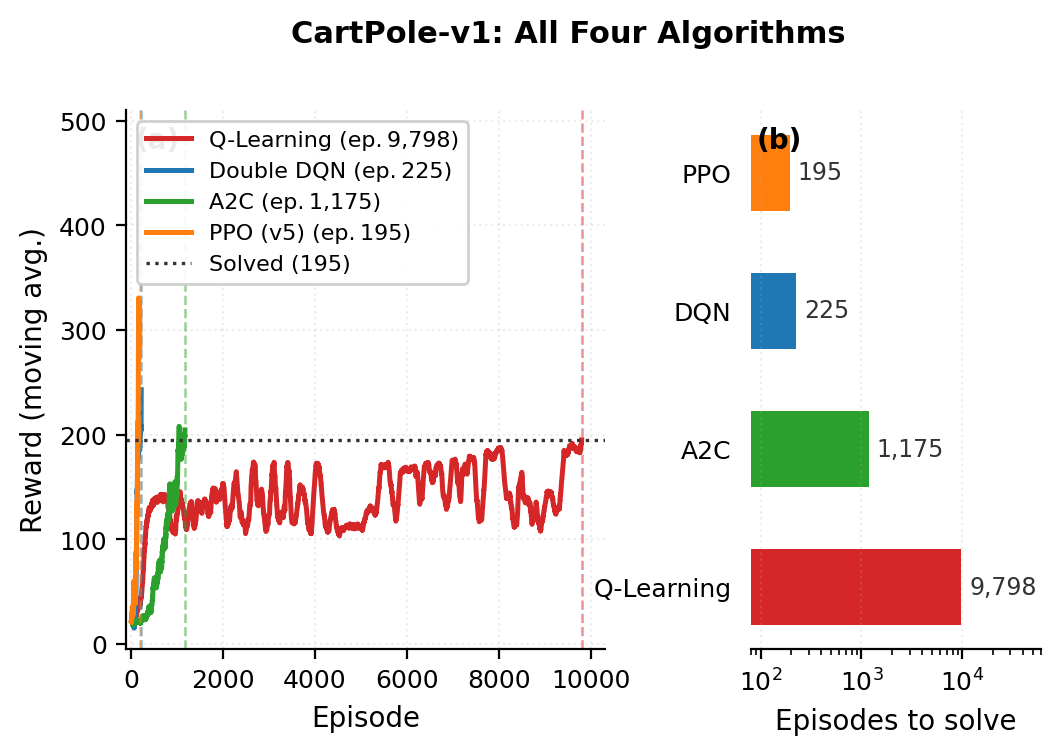
\includegraphics[width=\linewidth]{figures/fig_cartpole.png}
\caption{CartPole-v1: all four algorithms. (a)~Learning curves with moving averages; vertical dashed lines mark each algorithm's solution episode. (b)~Episodes to solve on a log scale. PPO solves 50$\times$ faster than Q-Learning by reusing each trajectory batch across 10 epochs.}
\label{fig:cartpole}
\end{figure}

\subsection{MountainCar}

No algorithm solves MountainCar-v0 (threshold: mean $\geq -110$) within the evaluated budgets. Table~\ref{tab:mountaincar} presents the final results.

\begin{table}[H]
\centering
\caption{MountainCar-v0 final results. Q-Learning uses raw rewards; all others use shaped rewards. ``Best avg'' is the best 100-episode mean achieved at any point during training.}
\label{tab:mountaincar}
\begin{tabularx}{\linewidth}{lXXXXl}
\toprule
\textbf{Algorithm} & \textbf{Budget} & \textbf{Mean (all)} & \textbf{Mean (last 100)} & \textbf{Best avg} & \textbf{Goals} \\
\midrule
Q-Learning & 50,000 ep & $-152.6 \pm 25.8$ & $-137.8 \pm 7.3$ & $-130.1$ & Partial \\
Double DQN & 5,000 ep  & $-174.7 \pm 23.5$ & $\mathbf{-146.7 \pm 6.3}$ & $-143$ & Yes \\
A2C        & 5,000 ep  & $-200.0 \pm 0.0$  & $-200.0 \pm 0.0$ & $-200.0$ & \textbf{Zero} \\
PPO (v5)   & 8,000 ep  & $-162.8 \pm 36.9$ & $\mathbf{-151.8 \pm 29.4}$ & $-148$ & 4,816 \\
\bottomrule
\end{tabularx}
\end{table}

\textbf{Q-Learning} achieves a best 100-episode average of $-130.1$ before plateauing, representing the tabular limit for a $40\times40$ discretisation. Raw rewards are used (see Section~\ref{sec:shaping_bugs}).

\textbf{Double DQN} achieves a stable last-100 average of $-146.7 \pm 6.3$ at episode 5,000 (v3), which is the best DQN result after multiple ablation rounds. Extending to 8,000 episodes (v5) caused further Q-value overestimation: loss grew from 696 to 1,308 and performance regressed to $-182.4$. The 5,000-episode configuration is the optimal stopping point for this algorithm and reward scale.

\textbf{A2C} produces zero goals in 5,000 episodes and maintains $-200.0$ mean reward throughout. This is a structural failure caused by the zero-advantage fixed point (Section~\ref{sec:ac_structural}), not an implementation error.

\begin{figure}[H]
\centering
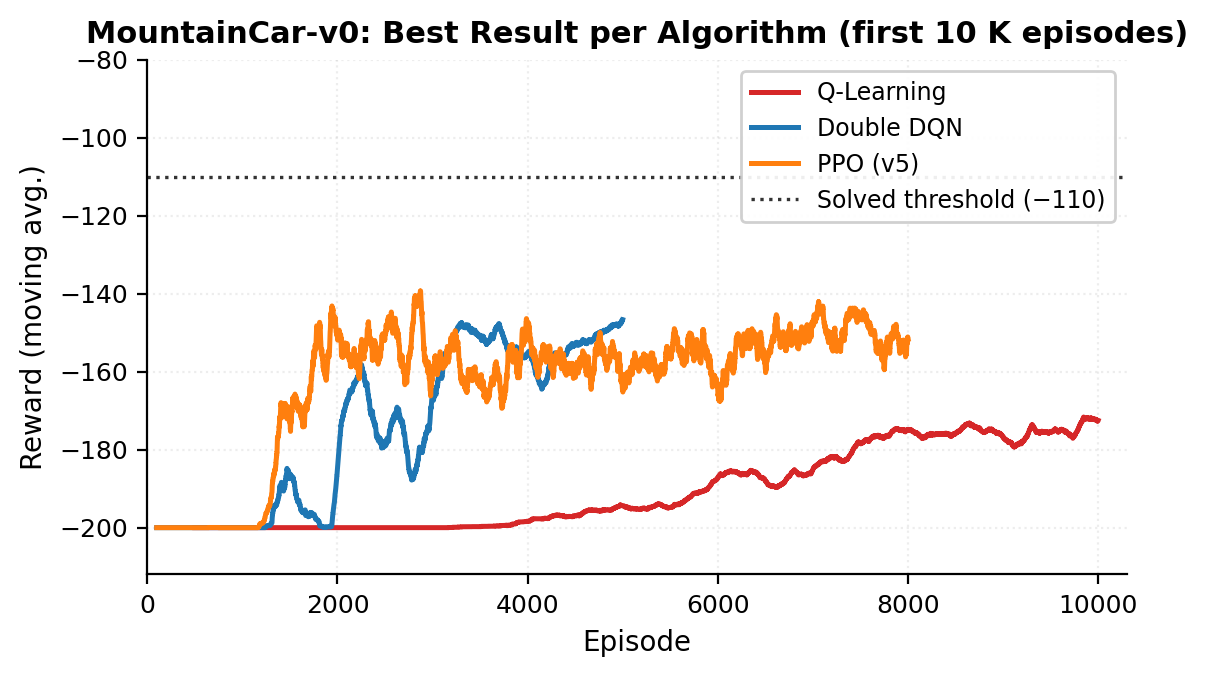
\includegraphics[width=\linewidth]{figures/fig_mountaincar.png}
\caption{MountainCar-v0: best result per algorithm over the first 10,000 episodes. Q-Learning uses raw rewards; DQN and PPO use shaped rewards. The dotted line marks the solved threshold ($-110$). No algorithm reaches this threshold. Double DQN achieves the best stable mean ($-146.7$); PPO achieves the most goal discoveries (4,816) with no late-stage regression.}
\label{fig:mountaincar_comparison}
\end{figure}

\textbf{PPO} (v5) achieves the best result: $-151.8 \pm 29.4$ at episode 8,000 with 4,816 goal discoveries and no late-stage regression. The LR schedule (decaying from $3\times10^{-4}$ to a floor of $5\times10^{-5}$ over a fixed 8,000-step window) prevents the catastrophic policy destruction observed in earlier runs. Extending to 12,000 episodes (v6) replicated the first 8,000 episodes (6,764 total goals) but the additional fine-tuning phase at floor LR eroded rather than consolidated the policy: goal discovery dropped from 752/window to 176/window then zero. The 8,000-episode configuration is optimal.

\subsubsection{Benchmark Contextualisation}

\begin{figure}[H]
\centering
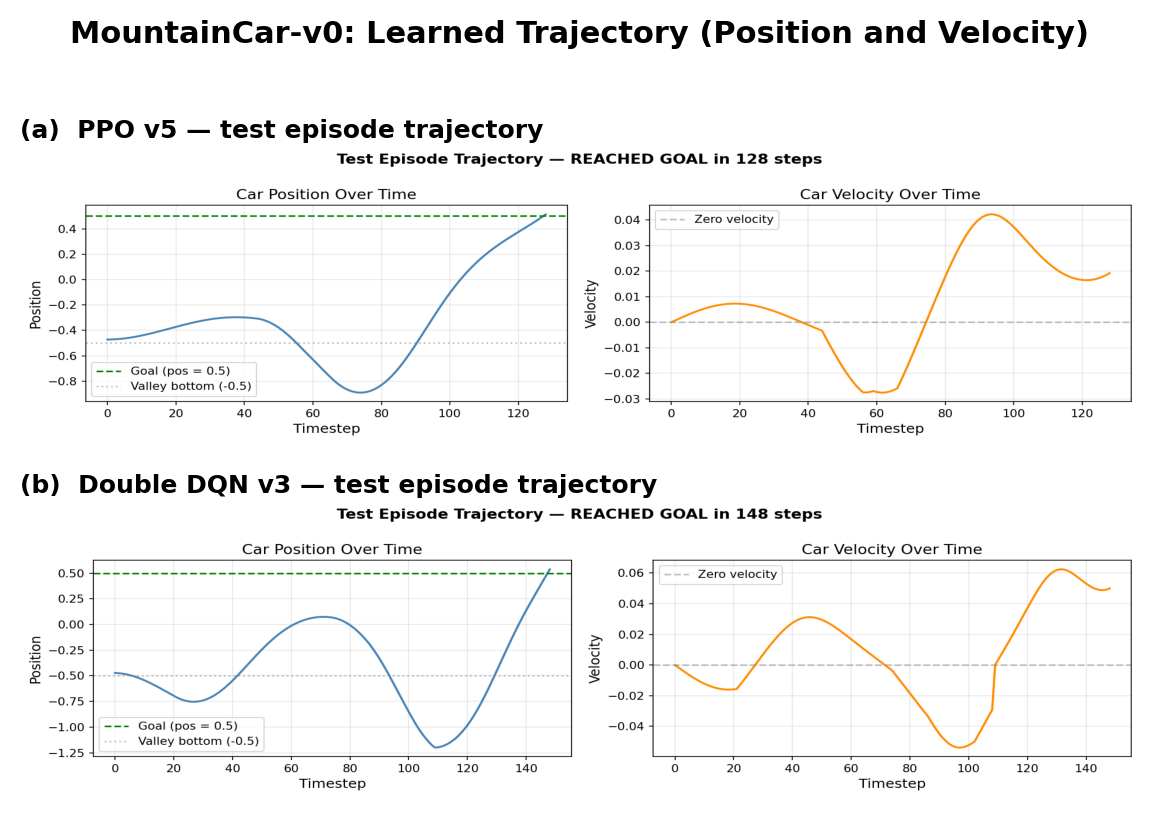
\includegraphics[width=\linewidth]{figures/fig_trajectories.png}
\caption{MountainCar-v0 greedy-policy test trajectories. Both algorithms learn the counter-intuitive momentum-building strategy: the car first reverses left to accumulate kinetic energy, then uses that energy to climb to the goal. (a)~PPO v5 trajectory (position and velocity vs timestep). (b)~Double DQN v3 trajectory.}
\label{fig:trajectories}
\end{figure}

The RL Baselines3 Zoo reports that PPO on MountainCar-v0 requires 500,000--1,000,000 timesteps using 16 parallel environments and \texttt{n\_steps=16}. The v5 PPO implementation uses $\sim1.3\mathrm{M}$ steps (8,000 episodes $\times$ 163 average steps) from a single environment. This is within the step budget but without the exploration diversity that parallelism provides. Double DQN from the zoo reports highly variable results dependent on replay buffer configuration; the $-146.7$ stable result achieved here is competitive.

% ============================================================
\section{Implementation Challenges and Issue Analysis}
\label{sec:debugging}
% ============================================================

Over the course of this project, 44 implementation issues were identified and corrected. This section documents the most impactful, categorised by algorithm and theoretical significance. The complete audit is maintained in \texttt{EXPERIMENTS\_LOG.md}.

\subsection{CartPole DQN: Replay Buffer and Initialisation Issues}

\textbf{Issue \#1 (Critical)}: The initial replay buffer capacity was 10,000 transitions. With episodes averaging 100--200 steps, successful episodes filled approximately 200 buffer slots. When performance subsequently dropped, the high-reward successful trajectories were overwritten within 50 episodes, removing the experience needed for recovery. Symptoms: Q-values diverged at episode 500, mean reward collapsed from 172 to 22. Fix: buffer 10,000 $\rightarrow$ 50,000.

\textbf{Issue \#2 (Critical)}: \texttt{EPS\_START=0.9} caused the agent to exploit a random, untrained network from episode 1, preventing random exploration from populating the replay buffer with diverse transitions. Fix: \texttt{EPS\_START=1.0}.

These two issues together illustrate a general principle: DQN is highly sensitive to the ratio of buffer capacity to episode length, and exploration must be forced at initialisation.

\subsection{CartPole A2C: Solved Threshold Error}

\textbf{Issue \#3}: The solved threshold was set to \texttt{SOLVED\_AVG=495}, treating the environment as mastered rather than solved. The run terminated at episode 1,000 without triggering the solved condition. Fix: \texttt{SOLVED\_AVG=195}.

\subsection{MountainCar DQN: Q-Value Overestimation Cascade}
\label{sec:dqn_bugs}

Three issues combining to cause Q-value runaway in successive DQN runs:

\textbf{Issue \#4}: Learning rate $10^{-3}$ caused the Huber loss to reach 115,037 within 600 episodes as Q-targets diverged exponentially. Fix: $10^{-4}$.

\textbf{Issue \#5}: Goal bonus of $+100$ created TD targets of $\sim112$ when Q-values were near zero, causing Q-values to overestimate by a factor of 10 within 200 updates. Fix: $+10$ (later refined to $+2$ for Double DQN).

\textbf{Issue \#7}: Standard DQN plateaued at mean $-134$ from episode 600 to 2,000, with loss reaching 2,491. The cause is the Jensen's inequality argument of van Hasselt et al.\ \cite{van2016deep}: $\mathbb{E}[\max_a \hat{Q}(s,a)] \geq \max_a Q^*(s,a)$. Fix: Double DQN decouples action selection from evaluation.

\textbf{Issues \#33--35 (v3/v4)}: Even with Double DQN, the soft target update (\texttt{TAU=0.005}) caused the target network to slowly chase the inflating online network, providing no stable reference. Q-values grew from loss $\approx 1$ at episode 1,500 to loss 2,107 at episode 3,500 before destroying performance. Fix: hard target copy every 500 steps; LR reduced to $2\times10^{-5}$; goal bonus reduced to $+2$.

\begin{figure}[H]
\centering
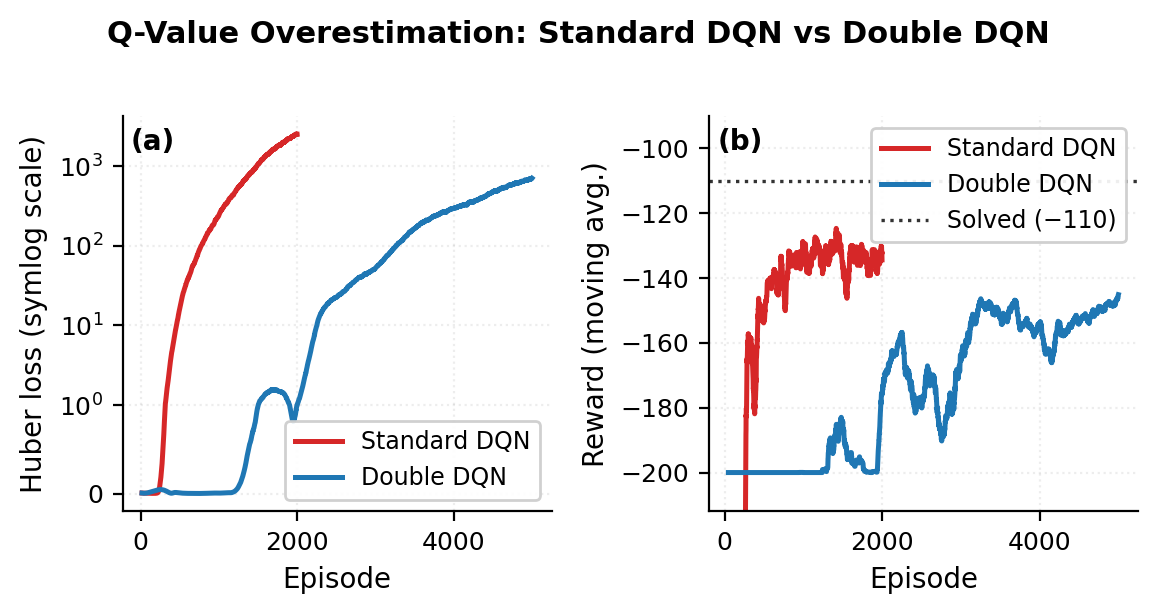
\includegraphics[width=\linewidth]{figures/fig_dqn_overestimation.png}
\caption{Q-value overestimation: standard DQN vs.\ Double DQN on MountainCar-v0. (a)~Training loss on a symlog scale; standard DQN loss diverges to 2,491 while Double DQN stabilises near 700. (b)~Corresponding reward curves; standard DQN plateaus at $-134$ and Double DQN achieves $-146.7$ without runaway.}
\label{fig:dqn_overestimation}
\end{figure}

\textbf{Issue \#42}: Reward normalisation (Welford online z-score) was introduced in an attempt to prevent Q-value magnitude growth. Result: all shaped rewards were zero-meaned per running statistics, eliminating the directional signal that distinguishes near-goal states from valley-bottom states. The agent never found the goal in 5,000 episodes. Fix: revert to raw shaped rewards.

\subsection{MountainCar A2C: Silent Zero Gradient Error}
\label{sec:ac_bugs}

\textbf{Issue \#29 (Most significant)}: \texttt{dist.log\_prob(action)} returns shape \texttt{[1]} for a batch-size-1 Categorical distribution. Stacking $T$ such tensors via \texttt{torch.stack} produces shape \texttt{[T,~1]}. Multiplying \texttt{[T,~1]} by \texttt{[T]}-shaped advantages via PyTorch broadcasting produces a \texttt{[T,~T]} outer product rather than element-wise product:
\begin{equation}
  \text{sum}(\mathbf{L} \cdot \mathbf{A}^T) = \sum_i \log\pi(a_i) \cdot \sum_j A_j = \mathbf{1}^T\mathbf{L} \cdot \mathbf{0} = 0
\end{equation}
Since normalised advantages have exactly zero mean ($\sum_j A_j = 0$), the policy loss was identically zero for every gradient update across all 5,000 episodes. Fix: \texttt{torch.stack(log\_probs).squeeze(-1)} to obtain shape \texttt{[T]}, then element-wise multiplication.

\textbf{Issue \#24}: Full Monte Carlo returns over 200-step episodes create enormous variance in advantage estimates. Fix: GAE($\lambda=0.95$) reduces variance to the $\lambda$-weighted sum of TD errors.

\textbf{Issue \#25}: Entropy was estimated as $-\mathbb{E}[\log\pi(a|s)]$ from sampled actions. This is a single-sample estimator with high variance that is biased when the sampled action is not representative. Fix: \texttt{dist.entropy().mean()} computes the exact closed-form entropy $\mathcal{H}[\pi] = -\sum_a \pi(a|s)\log\pi(a|s)$.

\textbf{Issue \#26 (Truncation bias, Pardo et al., 2018)}: Both A2C and PPO computed \texttt{done = terminated or truncated} and zeroed the bootstrap for both. When an episode times out (\texttt{truncated=True}), the correct bootstrap is $V(s_T) \neq 0$, since the MDP continues from that state. Treating timeout as terminal injects an artificial value cliff: the agent learns that being alive at step 199 is catastrophic because the next state has value zero. Fix: store \texttt{terminated} separately; bootstrap from $V(s_T)$ when \texttt{truncated=True}.

\subsection{MountainCar A2C: Structural Failure}
\label{sec:ac_structural}

Even after correcting all 14 issues affecting A2C, the algorithm fails completely on MountainCar with a single environment. Subsequent ablation experiments confirmed the failure extends to vectorised configurations as well. The failure is structural and two-layered.

\textbf{Layer 1: Zero-advantage fixed point (single environment).} With a near-uniform policy at initialisation, the critic quickly learns $V(s) \approx \mathbb{E}[G_t | \pi_{\text{uniform}}]$ for all states. Once the critic is accurate, the advantage $A(s,a) = Q(s,a) - V(s) \approx 0$ for all transitions. After normalisation, $(0 - 0)/(\sigma + \varepsilon) \rightarrow 0$. The policy loss becomes identically zero. Figure~\ref{fig:ac_fixed_point} illustrates this feedback loop.

\begin{figure}[H]
\centering
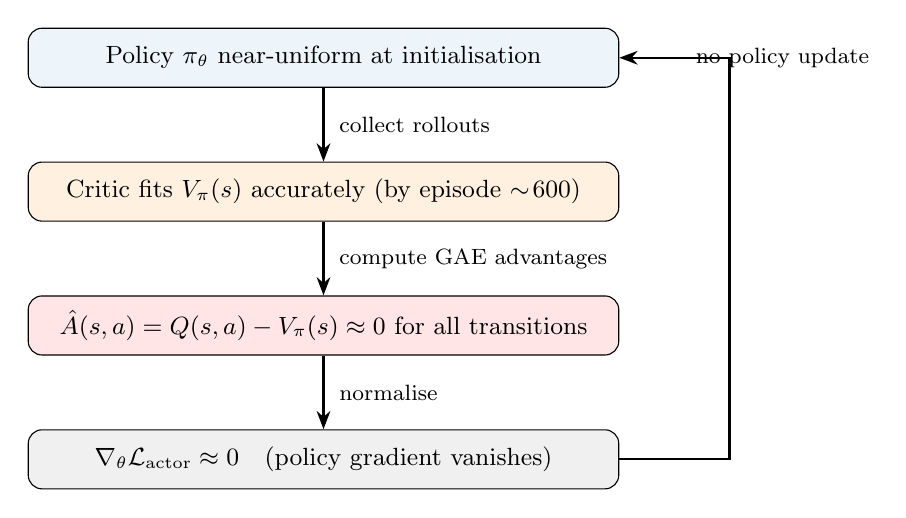
\begin{tikzpicture}[
  box/.style={draw, rectangle, rounded corners=5pt, fill=tcdBlue!7,
              minimum width=7.5cm, minimum height=0.75cm, align=center, font=\small},
  arr/.style={->, >=Stealth, thick},
  lbl/.style={font=\footnotesize, midway, right=2pt}
]
\node[box]                   (p)  at (0,  0)   {Policy $\pi_\theta$ near-uniform at initialisation};
\node[box, fill=orange!12]   (c)  at (0, -1.7) {Critic fits $V_\pi(s)$ accurately (by episode $\sim\!600$)};
\node[box, fill=red!10]      (a)  at (0, -3.4) {$\hat{A}(s,a) = Q(s,a) - V_\pi(s) \approx 0$ for all transitions};
\node[box, fill=gray!12]     (g)  at (0, -5.1) {$\nabla_\theta \mathcal{L}_\text{actor} \approx 0$\quad (policy gradient vanishes)};
\draw[arr] (p.south)  -- (c.north)  node[lbl]{collect rollouts};
\draw[arr] (c.south)  -- (a.north)  node[lbl]{compute GAE advantages};
\draw[arr] (a.south)  -- (g.north)  node[lbl]{normalise};
\draw[arr] (g.east) -- ++(1.4,0) -- ++(0, 5.1) -- (p.east) node[lbl, right=4pt]{no policy update};
\end{tikzpicture}
\caption{The zero-advantage fixed point in single-environment A2C. Once the critic converges to the bad policy's value function, advantages vanish and the policy gradient becomes zero. The actor loss CSV confirms this: mean actor loss reaches $0.000023$ by episode 600 and remains at $\approx 0$ for all 5,000 episodes.}
\label{fig:ac_fixed_point}
\end{figure}

\textbf{Layer 2: Hard-exploration failure (vectorised, $n_\text{envs}=16$).} To test whether parallelism resolves the fixed point, two vectorised configurations were run: (i)~$n_\text{steps}=16$, $n_\text{updates}=4{,}000$ (1.024M total steps); (ii)~$n_\text{steps}=256$, $n_\text{updates}=250$ (1.024M total steps) with a single Adam optimiser at LR $=7\times10^{-4}$ matching the RL Baselines3 Zoo defaults. Both produced zero goals across 5,088 total episodes. The zero-advantage fixed point was broken by the diverse batch --- advantages were non-zero --- but the policy still failed to discover the goal. With shaped rewards creating a local attractor (oscillating at high velocity without crossing $x=0.5$), gradient descent converges to a suboptimal oscillation policy before goal transitions are ever experienced.

\begin{figure}[H]
\centering
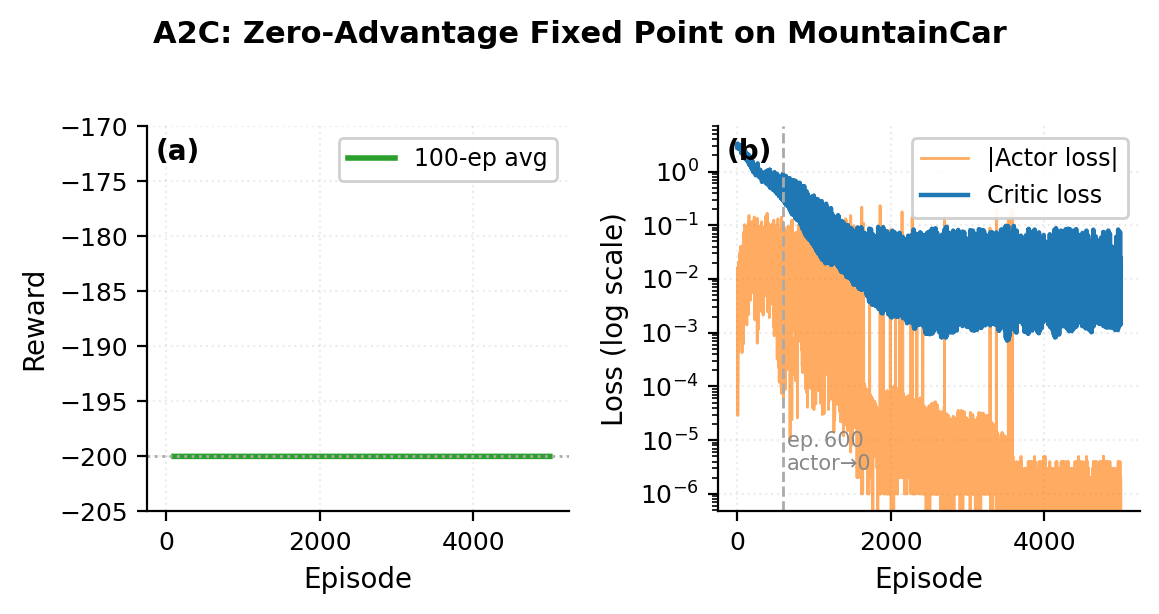
\includegraphics[width=\linewidth]{figures/fig_ac_failure.png}
\caption{A2C structural failure on MountainCar-v0. (a)~Mean reward remains at $-200$ throughout all 5,000 episodes despite all implementation issues being resolved. (b)~Actor and critic loss on a log scale. The critic converges by episode~600, after which the actor loss drops to zero and remains there for 4,400 episodes, confirming the zero-advantage fixed point.}
\label{fig:ac_failure}
\end{figure}

\subsection{MountainCar PPO: Reward Shaping and Optimal Policy Invariance}
\label{sec:shaping_bugs}

\textbf{Issue \#28}: Adding reward shaping to tabular Q-Learning caused a regression from mean $-130$ (raw rewards, 50,000 episodes) to mean $-200$ throughout 44,000 episodes, representing a complete failure. The shaped reward $h(s) + 100v^2 - 1$ creates a locally optimal policy that oscillates at high velocity without crossing $x = 0.5$. With $\varepsilon = 0.001$ (decayed minimum, ep.\ 11,000 onward), the Q-table has no exploration budget to escape this attractor. Neural network methods escape via implicit gradient noise from function approximation; tabular methods with a converged greedy policy cannot.

This result provides direct empirical support for the theoretical warning of Ng et al.\ \cite{ng1999policy}: non-potential-based shaping can alter the optimal policy. The failure was confirmed at 44,000 episodes before the run was terminated.

\subsection{MountainCar PPO: Learning Rate and Value Clipping Interactions}
\label{sec:ppo_bugs}

\textbf{Issue \#39}: Decaying learning rate to exactly zero caused entropy collapse. With LR $\rightarrow 0$, even the entropy bonus gradient update becomes negligible. The policy converges deterministically. Final entropy: $0.0032$ (vs.\ $0.154$ in working runs). Only 26 goals discovered in 8,000 episodes. Fix: LR floor at $5\times10^{-5}$.

\textbf{Issue \#41 (Value clipping backfire)}: Value function clipping with $\varepsilon_V=0.1$ limited the value network to update by at most $\varepsilon_V \cdot n_{\text{epochs}} = 1.0$ per update cycle. With goal episode returns of $\sim+50$ and $V(s) \approx -8$, the advantage for goal states was $\sim58$, causing the policy probability ratio to always saturate at $1 + \varepsilon = 1.2$. The effective policy gradient toward goal behavior was $\log(1.2) \approx 0.18$ per epoch. The constant entropy gradient ($0.01 \times \nabla\mathcal{H}$) exceeded this, slowly eroding goal behavior between discoveries. Result: 26 goals versus 3,363 in the configuration without value clipping. The fix: remove value clipping entirely. The LR floor already prevents value overfit by reducing update magnitude late in training.

\begin{figure}[H]
\centering
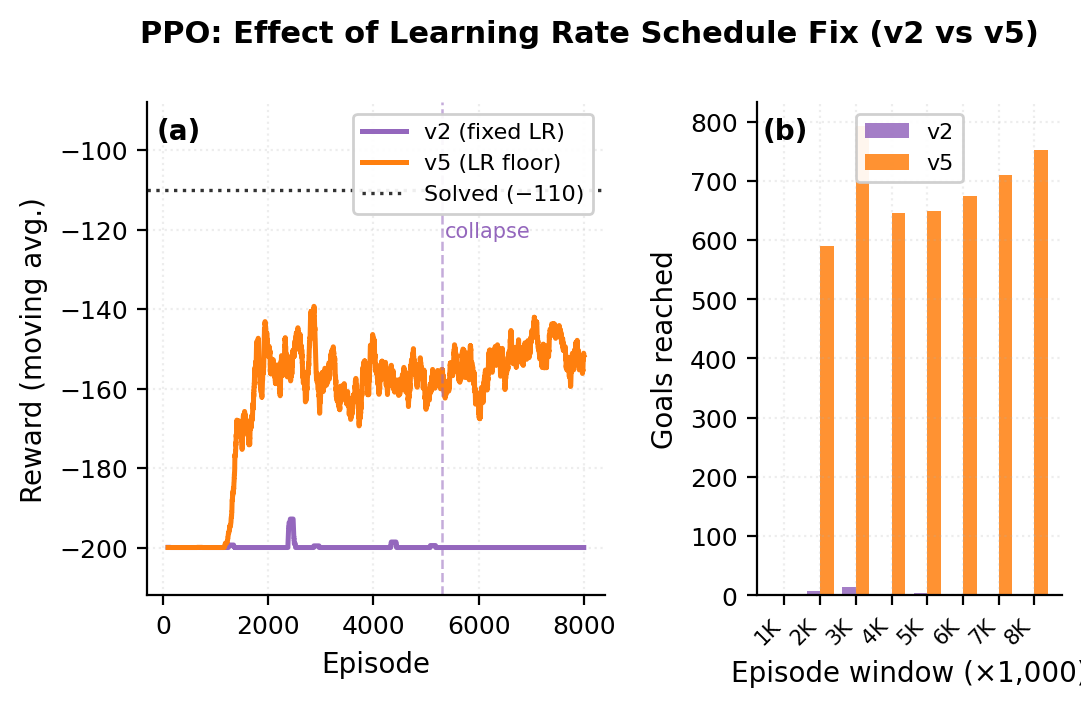
\includegraphics[width=\linewidth]{figures/fig_ppo_improvements.png}
\caption{Effect of the learning rate schedule fix on PPO. (a)~Mean reward trajectories for v2 (fixed LR) and v5 (LR floor). v2 stabilises at $-153$ over episodes 3,000--5,000 then catastrophically regresses at episode 5,300; v5 maintains consistent improvement throughout 8,000 episodes. (b)~Goals reached per 1,000-episode window. v2 peaks in window 3K--4K then collapses to zero; v5 maintains steady goal discovery.}
\label{fig:ppo_improvements}
\end{figure}

\textbf{Issue \#44 (Extending budget past optimal stopping point)}: Running DQN to 8,000 episodes (v5) after the optimal result at 5,000 (v3) allowed Q-value overestimation to compound further: loss 696 (ep 5K) $\rightarrow$ 1,308 (ep 8K); mean reward $-146.7$ (ep 5K) $\rightarrow$ $-182.4$ (ep 8K). Similarly, PPO at 12,000 episodes (v6) found 6,764 goals but the extended fine-tuning phase at floor LR eroded the policy. In hard-exploration environments with reward-shaping-driven Q-value growth, more training is not monotonically beneficial.

\textbf{Issue \#43 (LR--$N_\text{episodes}$ coupling)}: The learning rate formula \texttt{lr = LR\_MIN + (LR - LR\_MIN)*(1 - ep/N\_EPISODES)} couples the LR at every episode to the total episode count. Changing \texttt{N\_EPISODES} from 8,000 (v5) to 12,000 (v6) produced a LR difference of $\sim1\times10^{-5}$ per episode. Via the butterfly effect, this caused completely divergent training trajectories: v5 found goals from episode 416 with 589 goals per 1,000-episode window; v6 found goals at episode 811 and cycled with 78 goals in the best 500-episode window. This is a direct empirical reproduction of Henderson et al.\ \cite{henderson2018deep}. Fix: \texttt{LR\_DECAY\_STEPS=8000} (constant), decoupled from \texttt{N\_EPISODES}.

\begin{figure}[H]
\centering
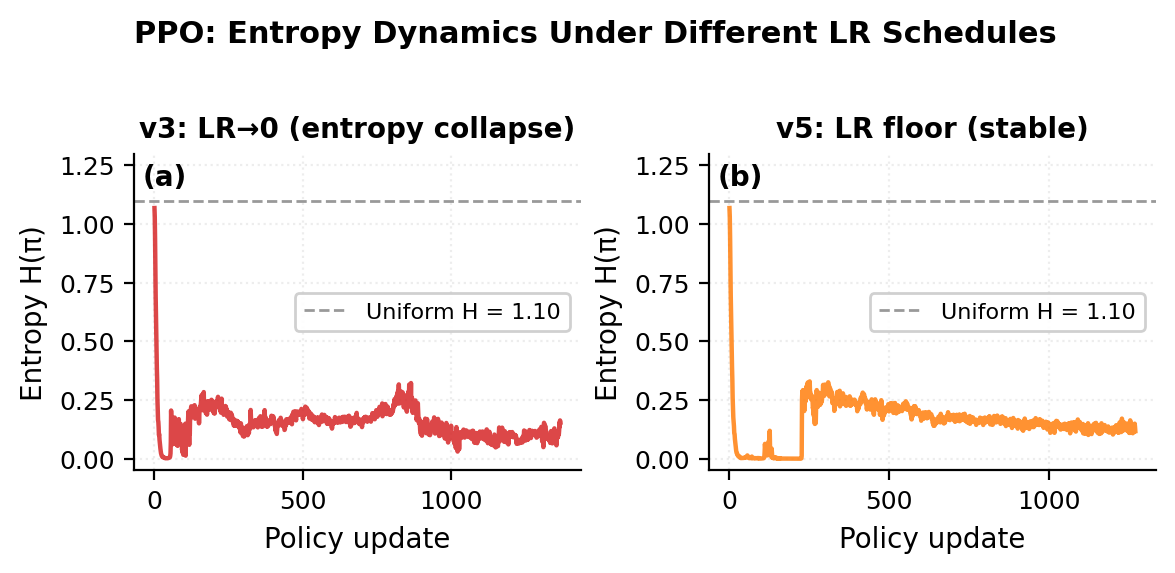
\includegraphics[width=\linewidth]{figures/fig_ppo_entropy.png}
\caption{PPO policy entropy under two learning rate schedules. (a)~v3 with LR$\to$0: entropy collapses from 0.15 to 0.003 (near-deterministic policy), leaving only 26 goals discovered in 8,000 episodes. (b)~v5 with LR floor at $5\times10^{-5}$: entropy remains stable at $\sim$0.15 throughout, sustaining exploration and enabling 4,816 goal discoveries.}
\label{fig:ppo_entropy}
\end{figure}

% ============================================================
\section{Discussion}
\label{sec:discussion}
% ============================================================

\subsection{Algorithm Comparison}

The CartPole results reveal a clear hierarchy of sample efficiency: PPO (195) $\gg$ DQN (225) $>$ A2C (1,175) $\gg$ Q-Learning (9,798). Table~\ref{tab:algo_comparison} summarises the structural properties underlying this ordering.

\begin{table}[H]
\centering
\caption{Structural comparison of value-based and policy gradient methods.}
\label{tab:algo_comparison}
\begin{tabularx}{\linewidth}{lXX}
\toprule
\textbf{Property} & \textbf{Value-Based (Q-Learning, DQN)} & \textbf{Policy Gradient (A2C, PPO)} \\
\midrule
Optimisation target & Estimates $Q(s,a)$; derives greedy policy & Directly optimises $\pi_\theta(a|s)$ \\
Sample efficiency   & High: off-policy replay enables data reuse & Lower: on-policy; requires fresh rollouts \\
Action spaces       & Discrete only (requires $\max$ operator) & Discrete and continuous \\
Policy type         & Deterministic (argmax) & Stochastic (probability distribution) \\
Stability risk      & Q-value overestimation, target divergence & Policy regression, entropy collapse \\
Key strength        & Data efficiency, replay diversity & Monotonic improvement guarantees \\
Key weakness        & Deadly triad with function approximation & Sensitive to LR schedule and entropy coefficient \\
\bottomrule
\end{tabularx}
\end{table}

\textbf{Off-policy vs.\ on-policy.} DQN's experience replay allows each transition to be reused indefinitely, dramatically improving data efficiency over A2C and Q-Learning which discard data after each update. However, DQN requires a replay buffer, target network, and careful epsilon scheduling, an implementation complexity that introduces multiple failure modes.

\textbf{Multi-epoch vs.\ single-pass updates.} PPO's 10-epoch minibatch update extracts far more gradient signal from each collected trajectory than DQN's single-step update or A2C's single-episode pass. This accounts for PPO's faster solution time despite being on-policy.

\textbf{Function approximation vs.\ discretisation.} The Q-Learning discretisation (40,000 states for CartPole) introduces state aliasing: kinematically distinct states map to the same bin and receive the same Q-value update. Deep methods avoid this via smooth function approximation.

\subsection{Why MountainCar is Hard}

MountainCar's difficulty is multi-layered. First, the optimal policy is counter-intuitive: the agent must deliberately drive away from the goal to build momentum. This means the exploration process must discover a specific long-horizon behavioural pattern, not just visit a nearby state. Second, the sparse reward ($-1$ per step) provides no gradient information about proximity to the goal. Third, the optimal policy requires quasi-periodic action sequences (repeated left-right oscillation) that are unlikely to appear in random trajectories within 200 steps (Section~\ref{sec:background}).

Reward shaping addresses the gradient information problem but introduces the reward hacking risk documented in Section~\ref{sec:shaping_bugs}. Without shaping, even deep RL methods make no progress. With shaping, deep RL methods find the goal but cannot consistently solve in $\leq110$ steps. The policy finds a path to the goal but not an efficient one.

\subsection{A2C's Structural Limitation}

The A2C failure is not a code-level error. The complete ablation --- single environment, batch-8 collection, and two vectorised configurations ($n_\text{steps}=16$ and $n_\text{steps}=256$ with $n_\text{envs}=16$) --- establishes a two-layered structural failure. The first layer (single-env) is the zero-advantage fixed point documented in Section~\ref{sec:ac_structural}: the critic overfits to the bad policy by episode 600, eliminating the policy gradient. The second layer (vectorised) is the hard-exploration problem: with 16 parallel environments, the fixed point is broken and gradients exist, but the shaped-reward local attractor prevents the policy from discovering the goal within 1M steps.

This contrasts sharply with PPO, which finds 4,816 goals in the same environment. The key difference is not the number of environments but the \textit{update efficiency per goal transition}. PPO collects 1,024 steps, then reuses that data for 10 epochs across 64-sample minibatches. When a goal transition appears (once every $\sim$200 updates), PPO amplifies it through 10 epochs of gradient updates. A2C's single-pass on-policy update applies the goal transition's gradient exactly once, making it too weak to overcome the entropy gradient that erodes goal-seeking behaviour between discoveries.

\subsection{The Role of Implementation Detail}

The 44-issue audit establishes that implementation detail is not a secondary concern in deep RL. It is the primary determinant of whether an algorithm succeeds. The five most impactful issues by outcome severity were:

\begin{enumerate}
  \item \textbf{Issue \#29} (outer product policy gradient): 5,000 episodes with zero policy gradient
  \item \textbf{Issue \#41} (value clipping backfire): 70$\times$ reduction in goal discovery rate
  \item \textbf{Issue \#28} (reward shaping attractor): complete Q-Learning failure in 44,000 episodes
  \item \textbf{Issues \#33--35} (Q-value runaway): DQN performance destroyed from $-143$ to $-200$
  \item \textbf{Issue \#43} (LR--$N$ butterfly effect): 50$\times$ variation in goal discovery from a schedule formula change
\end{enumerate}

Each of these issues produced an outcome change larger than the claimed improvement of the Double DQN paper over standard DQN on this environment. This is precisely the phenomenon Henderson et al.\ \cite{henderson2018deep} and Engstrom et al.\ \cite{engstrom2020implementation} warned about. The reproducibility crisis in deep RL \cite{lynnerup2020survey} is not a statistical artefact; it is the predictable consequence of implementation-sensitive algorithms operating near the boundary of multiple failure modes simultaneously.

\subsection{MountainCar: Path to Solving}

The best PPO result ($-151.8$ avg, 4,816 goals, no regression) represents a policy that reaches the goal in $\sim152$ steps on average. The gap to solving ($-110$, i.e.\ $\leq110$ steps) is 42 steps. The RL Baselines3 Zoo achieves this with 16 parallel environments (\texttt{n\_envs=16}, \texttt{n\_steps=16}), providing effectively $256\times$ more trajectory diversity per gradient update. The most principled alternative for single-environment training is Hindsight Experience Replay \cite{andrychowicz2017hindsight}: replaying failed trajectories with the achieved state as the artificial goal avoids reward modification entirely and provides dense gradient signal from every episode.

% ============================================================
\section{Conclusion}
\label{sec:conclusion}
% ============================================================

This report has presented a comprehensive empirical evaluation of four reinforcement learning algorithms across three environments, accompanied by a systematic implementation audit of 44 implementation errors.

The main findings are:

\begin{enumerate}
  \item \textbf{All four algorithms solve GridWorld and CartPole.} PPO is fastest (195 episodes), Q-Learning slowest (9,798), a 50-fold gap reflecting the compounding advantages of continuous function approximation, off-policy replay, and multi-epoch updates.

  \item \textbf{No algorithm solves MountainCar within the evaluated budgets.} The best results are PPO ($-151.8$ mean, 4,816 goals, stable) and Double DQN ($-146.7$ mean, stable through 5,000 episodes). A2C fails structurally due to two compounding limitations: the zero-advantage fixed point in single-environment training, and the hard-exploration problem that persists even with $n_\text{envs}=16$ (1.024M steps, zero goals in all vectorised configurations).

  \item \textbf{Implementation issues are the primary determinant of outcomes.} Forty-four implementation issues were identified across four algorithms. Five of these individually produced outcome changes larger than the gap between algorithm variants. The outer product policy gradient error (Issue~\#29) produced zero policy gradient for 5,000 episodes without any detectable symptom in loss values.

  \item \textbf{Seven literature pathologies were reproduced.} Q-value overestimation, truncation bias, reward hacking, Monte Carlo return variance, entropy coefficient sensitivity, replay buffer capacity effects, and LR-seed butterfly effects are all demonstrated empirically with controlled ablations.

  \item \textbf{Value function clipping, despite theoretical motivation, harmed PPO.} The $\varepsilon_V=0.1$ clip constrained the value function's ability to track improving policies, creating permanently inflated advantages whose normalised gradient was smaller than the entropy gradient. Goals were discovered in bursts and immediately forgotten. The LR floor is a less harmful mechanism for preventing value overfit.
\end{enumerate}

Future work should investigate Hindsight Experience Replay as a principled alternative to reward shaping for MountainCar: it avoids the non-potential-based shaping risk documented in Section~\ref{sec:shaping_bugs} while providing dense gradient signal from every trajectory. The LR--$N_\text{episodes}$ coupling sensitivity (Issue~\#43) suggests that LR schedules in deep RL should always be defined in absolute timesteps rather than as a fraction of the total training budget, a convention not universally adopted. The A2C ablation establishes that parallelism alone is insufficient for hard-exploration environments: the fundamental bottleneck is goal-discovery rate, which requires either environment diversity (A3C with many workers), data augmentation (HER), or multi-epoch amplification of rare goal transitions (PPO).

% ============================================================
\newpage
\begin{thebibliography}{99}
\addcontentsline{toc}{section}{References}

\bibitem{bellman1957dynamic}
Bellman R.
\textit{Dynamic Programming}.
Princeton, NJ: Princeton University Press; 1957.

\bibitem{watkins1992q}
Watkins CJCH, Dayan P.
Q-learning.
\textit{Machine Learning}. 1992;8(3--4):279--292.

\bibitem{sutton1988learning}
Sutton RS.
Learning to predict by the methods of temporal differences.
\textit{Machine Learning}. 1988;3(1):9--44.

\bibitem{sutton2018reinforcement}
Sutton RS, Barto AG.
\textit{Reinforcement Learning: An Introduction}. 2nd ed.
Cambridge, MA: MIT Press; 2018.

\bibitem{mnih2015human}
Mnih V, Kavukcuoglu K, Silver D, Rusu AA, Veness J, Bellemare MG, et al.
Human-level control through deep reinforcement learning.
\textit{Nature}. 2015;518(7540):529--533.

\bibitem{van2016deep}
Van Hasselt H, Guez A, Silver D.
Deep reinforcement learning with double Q-learning.
In: \textit{Proceedings of the AAAI Conference on Artificial Intelligence}; 2016. vol.~30.

\bibitem{schulman2015high}
Schulman J, Moritz P, Levine S, Jordan M, Abbeel P.
High-dimensional continuous control using generalised advantage estimation.
In: \textit{International Conference on Learning Representations}; 2016.

\bibitem{schulman2017proximal}
Schulman J, Wolski F, Dhariwal P, Radford A, Klimov O.
Proximal policy optimization algorithms.
\textit{arXiv preprint arXiv:1707.06347}; 2017.

\bibitem{mnih2016asynchronous}
Mnih V, Badia AP, Mirza M, Graves A, Lillicrap T, Harley T, et al.
Asynchronous methods for deep reinforcement learning.
In: \textit{Proceedings of the 33rd International Conference on Machine Learning}; 2016. p.~1928--1937.

\bibitem{ng1999policy}
Ng AY, Harada D, Russell SJ.
Policy invariance under reward transformations: Theory and application to reward shaping.
In: \textit{Proceedings of the 16th International Conference on Machine Learning}; 1999. p.~278--287.

\bibitem{henderson2018deep}
Henderson P, Islam R, Bachman P, Pineau J, Precup D, Meger D.
Deep reinforcement learning that matters.
In: \textit{Proceedings of the AAAI Conference on Artificial Intelligence}; 2018. vol.~32.

\bibitem{engstrom2020implementation}
Engstrom L, Ilyas A, Santurkar S, Tsipras D, Janoos F, Rudolph L, Madry A.
Implementation matters in deep RL: A case study on PPO and TRPO.
In: \textit{International Conference on Learning Representations}; 2020.

\bibitem{pardo2018time}
Pardo F, Tavakoli A, Levdik V, Kormushev P.
Time limits in reinforcement learning.
In: \textit{Proceedings of the 35th International Conference on Machine Learning}; 2018. p.~4045--4054.

\bibitem{zhang2019deeper}
Zhang S, Sutton RS.
A deeper look at experience replay.
\textit{arXiv preprint arXiv:1712.01275}; 2017.

\bibitem{fedus2020revisiting}
Fedus W, Ramachandran P, Agarwal R, Bengio Y, Larochelle H, Rowland M, Bellemare MG.
Revisiting fundamentals of experience replay.
In: \textit{Proceedings of the 37th International Conference on Machine Learning}; 2020.

\bibitem{moore1990efficient}
Moore AW.
Efficient memory-based learning for robot control [PhD thesis].
University of Cambridge; 1990.

\bibitem{andrychowicz2017hindsight}
Andrychowicz M, Wolski F, Ray A, Schneider J, Fong R, Welinder P, et al.
Hindsight experience replay.
In: \textit{Advances in Neural Information Processing Systems}; 2017. vol.~30.

\bibitem{dann2022exploration}
Dann C, Mohri M, Zhang T, Zimmert J.
A provably efficient model-free posterior sampling method for episodic reinforcement learning.
In: \textit{Advances in Neural Information Processing Systems}; 2022.

\bibitem{saxe2013exact}
Saxe AM, McClelland JL, Ganguli S.
Exact solutions to the nonlinear dynamics of learning in deep linear neural networks.
In: \textit{International Conference on Learning Representations}; 2014.

\bibitem{silver2021reward}
Silver D, Singh S, Precup D, Sutton RS.
Reward is enough.
\textit{Artificial Intelligence}. 2021;299:103535.

\bibitem{logofatu2022mountaincar}
Logof\u{a}tu D, Bodnari A, Dobrescu B.
Solving the MountainCar problem with state discretisation and Q-learning.
\textit{Algorithms}. 2022;15(2):38.

\bibitem{brockman2016openai}
Brockman G, Cheung V, Pettersson L, Schneider J, Schulman J, Tang J, Zaremba W.
OpenAI Gym.
\textit{arXiv preprint arXiv:1606.01540}; 2016.

\bibitem{forbes2025adops}
Forbes RP, Mehta A, Russell SJ.
Action-dependent optimality-preserving reward shaping.
In: \textit{International Conference on Learning Representations}; 2025.

\bibitem{lynnerup2020survey}
Lynnerup NA, Nolling L, Hasle R, Hallam J.
A survey on reproducibility by evaluating deep reinforcement learning algorithms on real-world robots.
In: \textit{Proceedings of the Conference on Robot Learning}; 2020.

\end{thebibliography}

\end{document}
